\section{Fanny Shafira Damayanti (1174069)}
\subsection{Teori}
\begin{enumerate}

\item Jelaskan apa itu binary classification dilengkapi ilustrasi gambar sendiri\\
Klasifikasi biner tugasnya yaitu untuk mengklasifikasikan elemen-elemen dari himpunan yang diberikan ke dalam dua kelompok berdasarkan aturan klasifikasi.

\begin{figure}[H]
		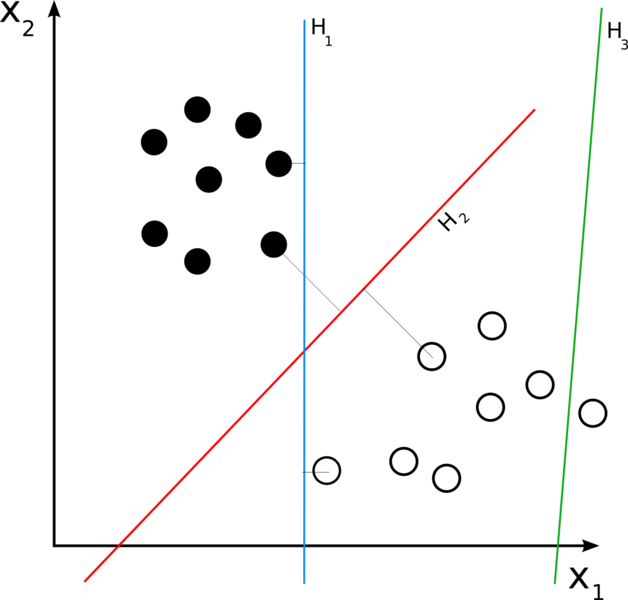
\includegraphics[width=4cm]{figures/1174069/2/binclass.png}
		\centering
		\caption{Binary Classification}
	\end{figure}

\item Jelaskan apa itu supervised learning dan unsupervised learning dan clustering dengan ilustrasi gambar sendiri\\

Supervised Learning adalah tipe learning di mana kita mempunyai variable input dan variable output, dan menggunakan satu algoritma atau lebih untuk mempelajari fungsi pemetaan dari input ke output.

\begin{figure}[H]
		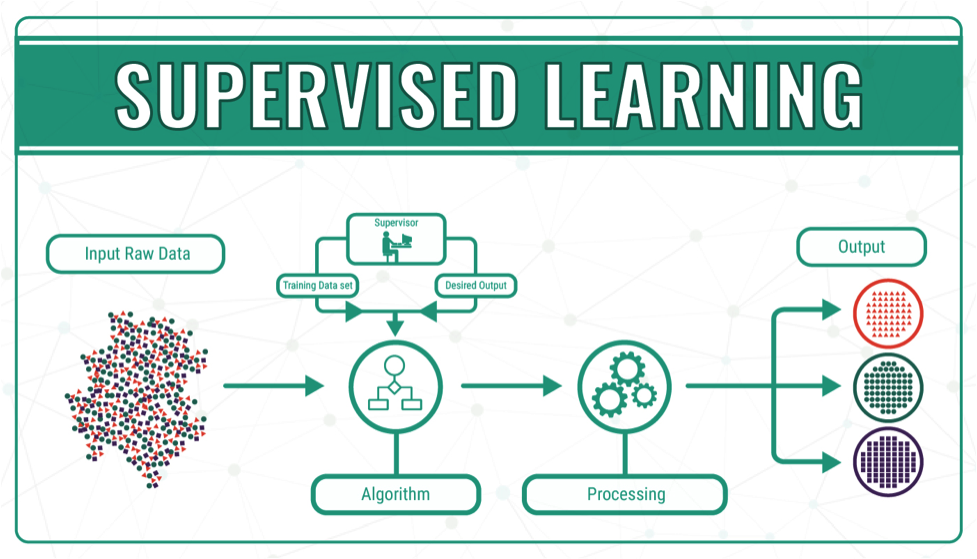
\includegraphics[width=4cm]{figures/1174069/2/sl.png}
		\centering
		\caption{Supervised Learning}
	\end{figure}
	
Unsupervised learning adalah tipe learning di mana kita hanya mempunyai data masukan (input data) tetapi tidak ada output variable yang berhubungan.

\begin{figure}[H]
		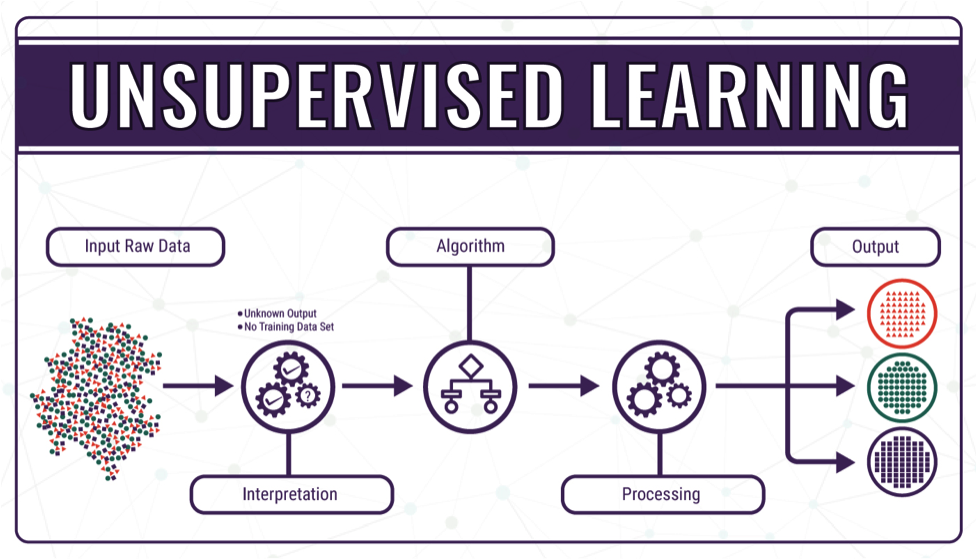
\includegraphics[width=4cm]{figures/1174069/2/usl.png}
		\centering
		\caption{Unsupervised learning}
	\end{figure}
	
Analisis atau pengelompokan klaster adalah tugas pengelompokan sekumpulan objek sedemikian rupa sehingga objek dalam kelompok yang sama lebih mirip satu sama lain daripada pada kelompok lain.

\begin{figure}[H]
		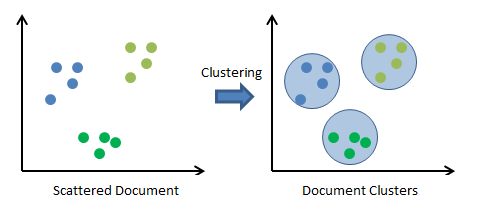
\includegraphics[width=4cm]{figures/1174069/2/clus.png}
		\centering
		\caption{Clustering}
	\end{figure}	
	
\item Jelaskan apa itu evaluasi dan akurasi dari buku dan disertai ilustrasi contoh dengan gambar sendiri\\

Evaluasi merupakan saduran dari bahasa Inggris "evaluation" yang diartikan sebagai penaksiran atau penilaian. Nurkancana (1983) menyatakan bahwa evaluasi adalah kegiatan yang dilakukan berkenaan dengan proses untuk menentukan nilai dari suatu hal.\\

Akurasi adalah derajat kesesuaian, yaitu tingkat yang mana pengukuran adalah tepat ketika dibandingkan dengan nilai absolut.

\item Jelaskan bagaimana cara membuat dan membaca confusion matrix, buat confusion matrix buatan sendiri.\\

Confusion matrix adalah suatu metode yang biasanya digunakan untuk melakukan perhitungan akurasi pada konsep data mining atau Sistem Pendukung Keputusan. Pada pengukuran kinerja menggunakan confusion matrix, terdapat 4 (empat) istilah sebagai representasi hasil proses klasifikasi. Keempat istilah tersebut adalah True Positive (TP), True Negative (TN), False Positive (FP) dan False Negative (FN). Nilai True Negative (TN) merupakan jumlah data negatif yang terdeteksi dengan benar, sedangkan False Positive (FP) merupakan data negatif namun terdeteksi sebagai data positif. Sementara itu, True Positive (TP) merupakan data positif yang terdeteksi benar. False Negative (FN) merupakan kebalikan dari True Positive, sehingga data posifit, namun terdeteksi sebagai data negatif.

\begin{figure}[H]
		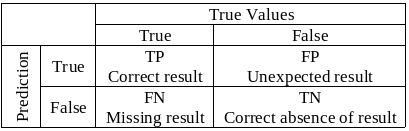
\includegraphics[width=4cm]{figures/1174069/2/cm.PNG}
		\centering
		\caption{Clustering}
	\end{figure}	

\item Jelaskan bagaimana K-fold cross validation bekerja dengan gambar ilustrasi contoh buatan sendiri.\\

Cross-validasi, atau bisa disebut estimasi rotasi, adalah sebuah teknik validasi model untuk menilai bagaimana hasil statistik analisis akan menggeneralisasi kumpulan data independen. Teknik ini utamanya digunakan untuk melakukan prediksi model dan memperkirakan seberapa akurat sebuah model prediktif ketika dijalankan dalam praktiknya. Dalam sebuah masalah prediksi, sebuah model biasanya diberikan kumpulan data (dataset) yang diketahui untuk digunakan dalam menjalankan pelatihan (dataset pelatihan), serta kumpulan data yang tidak diketahui (atau data yang pertama kali dilihat) terhadap model yang diuji (pengujian dataset).Tujuan dari validasi silang adalah untuk mendefinisikan dataset untuk "menguji" model dalam tahap pelatihan (yaitu, validasi data), dalam rangka untuk membatasi masalah seperti terjadinya overfitting, memberikan wawasan tentang bagaimana model akan menggeneralisasi independen dataset (yaitu, dataset tidak diketahui, misalnya dari masalah nyata), dll.

\begin{figure}[H]
		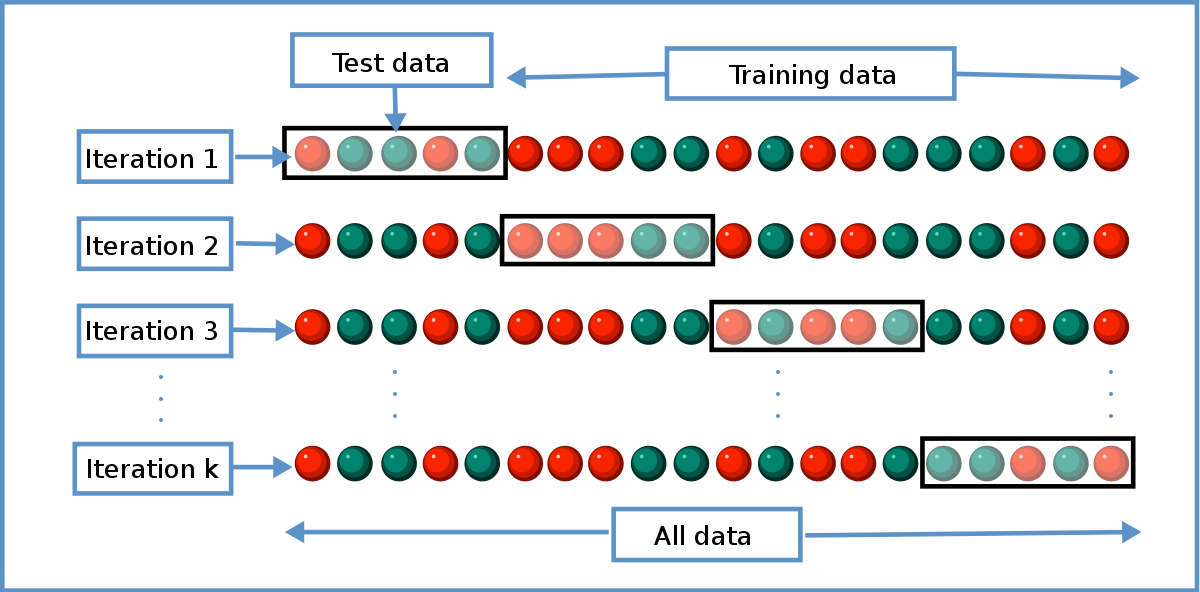
\includegraphics[width=4cm]{figures/1174069/2/kfold.png}
		\centering
		\caption{K-fold cross validation}
	\end{figure}
	
\item Jelaskan apa itu decision tree dengan gambar ilustrasi contoh buatan sendiri.\\

Pohon keputusan adalah alat pendukung keputusan yang menggunakan model keputusan seperti pohon dan konsekuensinya yang mungkin, termasuk hasil acara kebetulan, biaya sumber daya, dan utilitas. Ini adalah salah satu cara untuk menampilkan algoritma yang hanya berisi pernyataan kontrol bersyarat.

\begin{figure}[H]
		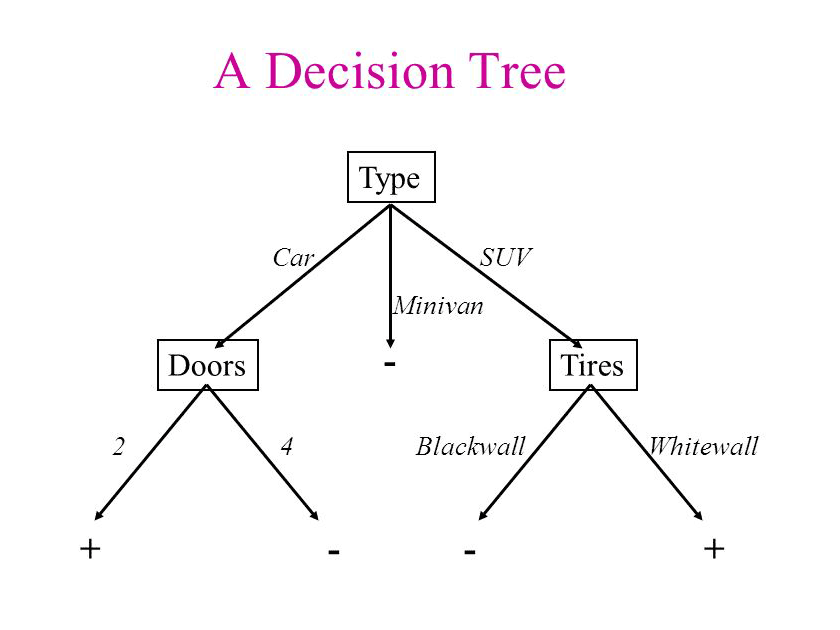
\includegraphics[width=4cm]{figures/1174069/2/dt.png}
		\centering
		\caption{Decision Tree}
	\end{figure}
	
\item Jelaskan apa itu information gain dan entropi dengan gambar ilustrasi buatan sendiri.\\

Metode Information Gain adalah metode yang menggunakan teknik scoring untuk pembobotan sebuah fitur dengan menggunakan maksimal entropy.

\begin{figure}[H]
		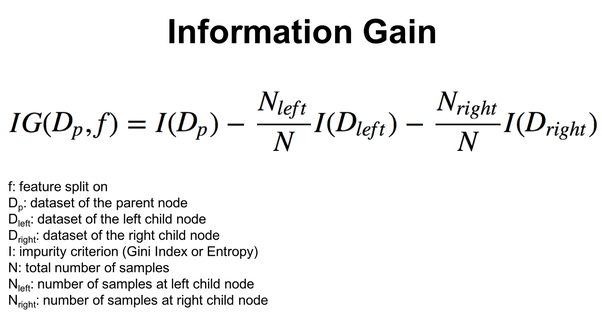
\includegraphics[width=4cm]{figures/1174069/2/ig.png}
		\centering
		\caption{Information Gain}
	\end{figure}
	
Entropi adalah salah satu besaran termodinamika yang mengukur energi dalam sistem per satuan temperatur yang tak dapat digunakan untuk melakukan usaha. 

\begin{figure}[H]
		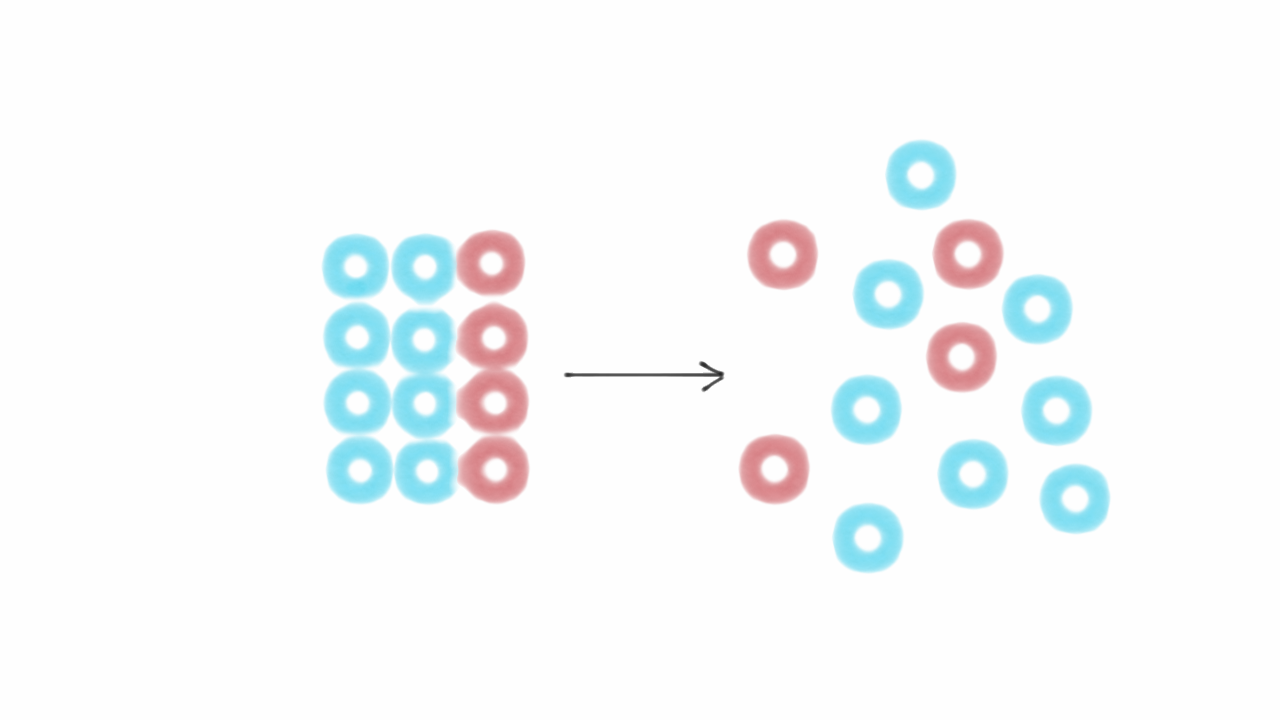
\includegraphics[width=4cm]{figures/1174069/2/Entropy.png}
		\centering
		\caption{Entropy}
	\end{figure}

\end{enumerate}

\subsection{scikit-learn}

\lstinputlisting[firstline=1, lastline=84]{src/1174069/2/1174069.py}

\subsection{Penganan Error}
\begin{enumerate}
\item Screenshoot Error

\begin{figure}[H]
		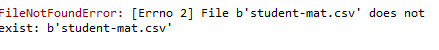
\includegraphics[width=4cm]{figures/1174069/2/error/error1.PNG}
		\centering
		\caption{File Not Found}
	\end{figure}
	
	\begin{figure}[H]
		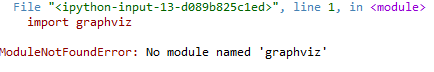
\includegraphics[width=4cm]{figures/1174069/2/error/error2.PNG}
		\centering
		\caption{Module Not Found}
	\end{figure}
	
	\begin{figure}[H]
		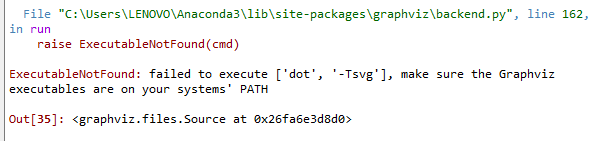
\includegraphics[width=4cm]{figures/1174069/2/error/error3.PNG}
		\centering
		\caption{Executable Not Found}
	\end{figure}
	
\item Jenis Error
	\begin{itemize}
	\item File Not Found
	\item Module Not Found
	\item Executable Not Found
	\end{itemize}
	
\item Solusi Error
\begin{itemize}
	\item File Not Found\\
	Mendownload filenya di github
	\begin{figure}[H]
		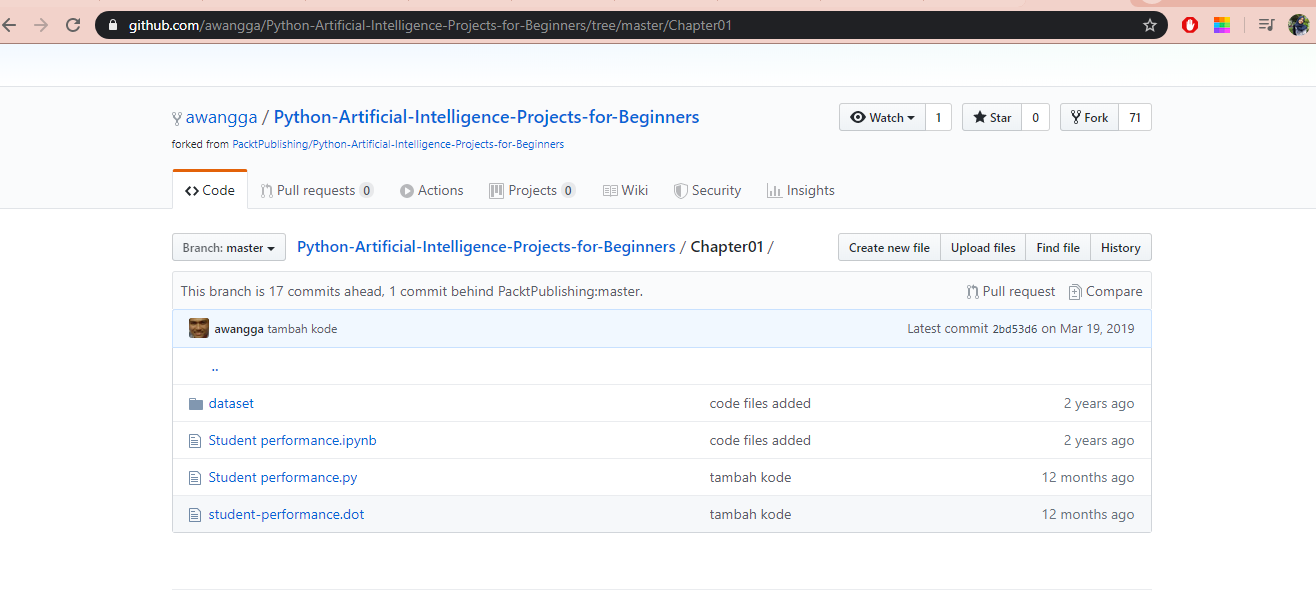
\includegraphics[width=4cm]{figures/1174069/2/error/solusi1.PNG}
		\centering
		\caption{File Dataset}
	\end{figure}
	
	\item Module Not Found\\
	Mendownload library graphviz menggunakan pip install graphviz di Anaconda Prompt
	\begin{figure}[H]
		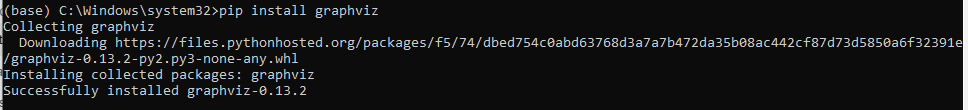
\includegraphics[width=4cm]{figures/1174069/2/error/solusi2.PNG}
		\centering
		\caption{Install graphviz}
	\end{figure}
	
	\item Executable Not Found
	Memasukkan PATH dari graphviz
	\lstinputlisting[firstline=42, lastline=43]{src/1174069/2/1174069.py}
	\end{itemize}
\end{enumerate}

\subsection{Scan Plagiarisme}
\begin{figure}[H]
		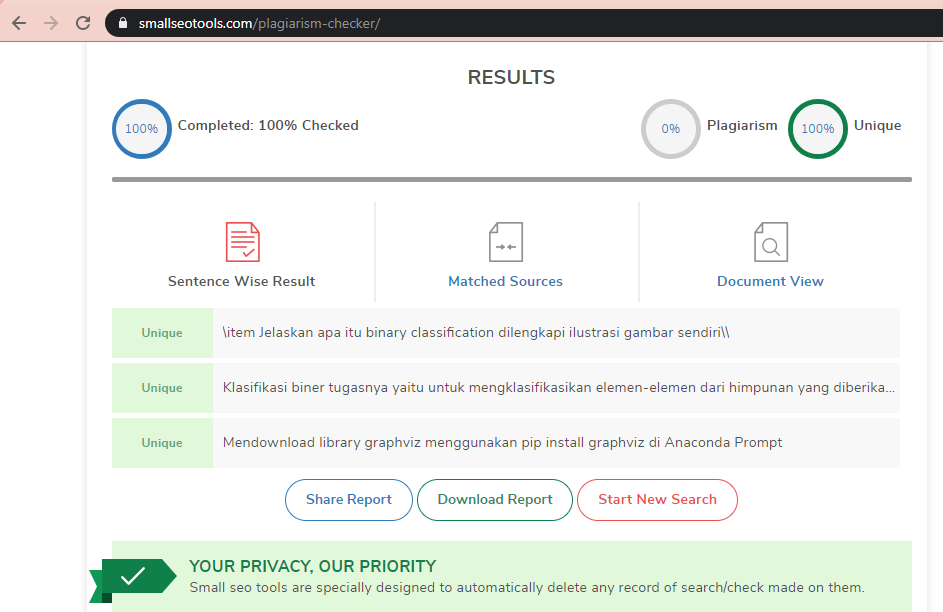
\includegraphics[width=4cm]{figures/1174069/2/plagiarisme/plagiarisme.PNG}
		\centering
		\caption{Scan plagiarisme}
	\end{figure}
	
\subsection{Link Youtube}	
https://youtu.be/ZLN9sCwl9-I